% options:
% thesis=B bachelor's thesis
% thesis=M master's thesis
% czech thesis in Czech language
% slovak thesis in Slovak language
% english thesis in English language
% hidelinks remove colour boxes around hyperlinks

\documentclass[thesis=B,czech]{FITthesis}[2012/06/26]

\usepackage[utf8]{inputenc} % LaTeX source encoded as UTF-8

\usepackage{graphicx} % graphics files inclusion
\usepackage{amsmath} % advanced maths
\usepackage{amssymb} % additional math symbols

\usepackage{dirtree} % directory tree visualisation

% % list of acronyms
\usepackage[acronym,nonumberlist,toc,numberedsection=autolabel]{glossaries}
\iflanguage{czech}{\renewcommand*{\acronymname}{Seznam pou{\v z}it{\' y}ch zkratek}}{}
\makeglossaries

\newcommand{\tg}{\mathop{\mathrm{tg}}} %cesky tangens
\newcommand{\cotg}{\mathop{\mathrm{cotg}}} %cesky cotangens

% % % % % % % % % % % % % % % % % % % % % % % % % % % % % % 
% ODTUD DAL VSE ZMENTE
% % % % % % % % % % % % % % % % % % % % % % % % % % % % % % 

%%%%%%%%%%%%%%%%%%%%%%%%%%%%%%%%%%%%%%%%%%%%%%%%%%%%%%%%%%%% <nesrotom>

\providecommand{\e}[1]{\ensuremath{\times 10^{#1}}}

\usepackage{float}

\usepackage{algorithm}% http://ctan.org/pkg/algorithms
\usepackage{algpseudocode}% http://ctan.org/pkg/algorithmicx
\usepackage{pseudocode}

\let\mylistof\listof
\renewcommand\listof[2]{%
\mylistof{algorithm}{Seznam algoritmů}%
}

% macro to define a local label
%\newcommand\locallabel[1]{\label{\currentprefix:#1}}
% macro to use a local reference
%\newcommand\localref[1]{\ref{\currentprefix:#1}}

%\mylistof{algorithm}{}

%%%%%%%%%%%%%%%%%%%%%%%%%%%%%%%%%%%%%%%%%%%%%%%%%%%%%%%%%%%% </nesrotom>

\department{Katedra \ldots (DOPLŇTE)}
\title{Doplňte název práce}
\authorGN{Doplňte Vaše křestní jméno/jména} %(křestní) jméno (jména) autora
\authorFN{Doplňte Vaše příjmení} %příjmení autora
\authorWithDegrees{Doplňte Vaše jméno a tituly} %jméno autora včetně současných akademických titulů
\supervisor{Doplňte jméno vedoucího práce}
\acknowledgements{Doplňte, máte-li komu a za co děkovat. V~opačném případě úplně odstraňte tento příkaz.}
\abstractCS{V~několika větách shrňte obsah a přínos této práce v~češtině. Po přečtení abstraktu by se čtenář měl mít čtenář dost informací pro rozhodnutí, zda chce Vaši práci číst.}
\abstractEN{Sem doplňte ekvivalent abstraktu Vaší práce v~angličtině.}
\placeForDeclarationOfAuthenticity{V~Praze}
\declarationOfAuthenticityOption{4} %volba Prohlášení (číslo 1-6)
\keywordsCS{Nahraďte seznamem klíčových slov v češtině oddělených čárkou.}
\keywordsEN{Nahraďte seznamem klíčových slov v angličtině oddělených čárkou.}

\begin{document}

% \newacronym{CVUT}{{\v C}VUT}{{\v C}esk{\' e} vysok{\' e} u{\v c}en{\' i} technick{\' e} v Praze}
% \newacronym{FIT}{FIT}{Fakulta informa{\v c}n{\' i}ch technologi{\' i}}

\begin{introduction}
	%sem napište úvod Vaší práce
\end{introduction}

%%%%%%%%%%%%%%%%%%%%%%%%%%%%%%%%%%%%%%%%%%%%%%%%%%%%%%%%%%%%%%%%%%%%%%%%%%%%%%
%%%%%%%%%%%%%%%%%%%%%%%%%%%%%%%%%%%%%%%%%%%%%%%%%%%%%%%%%%%%%%%%%%%%%%%%%%%%%%
%%%%%%%%%%%%%%%%%%%%%%%%%%%%%%%%%%%%%%%%%%%%%%%%%%%%%%%%%%%%%%%%%%%%%%%%%%%%%%
%%%%%%%%%%%%%%%%%%%%%%%%%%%%%%%%%%%%%%%%%%%%%%%%%%%%%%%%%%%%%%%%%%%%%%%%%%%%%%
%%%%%%%%%%%%%%%%%%%%%%%%%%%%%%%%%%%%%%%%%%%%%%%%%%%%%%%%%%%%%%%%%%%%%%%%%%%%%%
%%%%%%%%%%%%%%%%%%%%%%%%%%%%%%%%%%%%%%%%%%%%%%%%%%%%%%%%%%%%%%%%%%%%%%%% begin
%%%%%%%%%%%%%%%%%%%%%%%%%%%%%%%%%%%%%%%%%%%%%%%%%%%%%%%%%%%%%%%%%%%%%%%%%%%%%%
%%%%%%%%%%%%%%%%%%%%%%%%%%%%%%%%%%%%%%%%%%%%%%%%%%%%%%%%%%%%%%%%%%%%%%%%%%%%%%
%%%%%%%%%%%%%%%%%%%%%%%%%%%%%%%%%%%%%%%%%%%%%%%%%%%%%%%%%%%%%%%%%%%%%%%%%%%%%%
%%%%%%%%%%%%%%%%%%%%%%%%%%%%%%%%%%%%%%%%%%%%%%%%%%%%%%%%%%%%%%%%%%%%%%%%%%%%%%
%%%%%%%%%%%%%%%%%%%%%%%%%%%%%%%%%%%%%%%%%%%%%%%%%%%%%%%%%%%%%%%%%%%%%%%%%%%%%%

\chapter{Úvod do problematiky}

\section{Použití násobení matic}

% inverze matic: Matrix multiplication and matrix inversion ItA

TODO: kde se pouziva nasobeni matic

\section{Matice}

Matice \textbf{A} typu ($m$, $n$) je $m n$ uspořádaných prkvů z množiny $\mathbf{R}$. O prvku $a_{r,s} \in \mathbf{R}, r \in \{1,2,\hdots,m\},s \in \{1,2,\hdots,n\}$ říkáme, že je na r-tém řádku a~s-tém sloupci matice \textbf{A}. Matici \textbf{A} zapisujeme do řádků a~sloupců takto:
\begin{align}
\mathbf{A}=\begin{pmatrix}
a_{1,1} & a_{1,2} & \cdots & a_{1,n} \\
a_{2,1} & a_{2,2} & \cdots & a_{2,n} \\
\vdots  & \vdots  & \ddots & \vdots  \\
a_{m,1} & a_{m,2} & \cdots & a_{m,n}
\end{pmatrix}
\end{align}

Matici \textbf{M} typu ($m$, $n$), kde všechny její prvky jsou rovny nule, nazýváme \textit{nulovou maticí.}

O~matici typu ($m$, $n$) budeme říkat, že je $m$~široká a~$n$~vysoká. Pokud o~matici řekneme že má velikost $n$, myslíme tím, že je typu ($n$, $n$).

\section{Vektor}

Matici \textbf{V} typu (1, n) nazveme vektorem.

TODO=popsat vektory poradne
FIXME=muzu to takhle zjednodusit?

\section{Násobení matic}

Buď \textbf{A} matice typu ($m$,$n$) s prvky $a_{i,j}$ a \textbf{B} matice typu ($n$,$p$) s prvky $b_{j,k}$. Definujeme součin matic $\mathbf{A} \cdot \mathbf{B}$ jako matici \textbf{C} typu ($m$,$p$) s prvky $c_{i,k}$ které vypočteme jako:

\begin{align}
c_{row,col}=\sum_{k=1}^{N} a_{row,k} b_{k,col}
\end{align}

Výsledek součinu matic se nezmění, pokud matice doplníme o~libovovolný počet nulových řádků a~nebo sloupců. Této vlastnosti můžeme využít pro získání potřebných rozměrů:

\begin{enumerate}
  \item Při násobení matice A typu ($m$,$n$) s maticí B typu ($o$,$p$), kde $ n \neq o $.
  \item Pokud potřebujeme matice stejné velikosti.
  \item Pokud potřebujeme matice určité velikosti, například $ 2^{ \mathbf{N}} $.
\end{enumerate}

\section{Složitosti}

TODO: popsat notace

% IntroductionToAlgoritms 3.1 asymptotic notations 43-97 (1217, 1222).

\section{Řídké matice}

Matice, které obsahují velké množství nulových prvků, nazýváme řídké. Nebudeme přesně uvádět kolik procent z celkového počtu prvků musí být nulových, abychom matici nazývali řídkou. Stejně jako řídkou matici můžeme uložit do formátu pro husté matice, můžeme hustou matici uložit do formátu pro řídké matice.

Řídkost matice budeme vyjadřovat pomocí $nnz$ (Number of NonZero elements), tedy počtem nenulových prvků z celkových $mn$, pro matici A typu ($m$, $n$).

TODO: typy ridkych matic (pasova, atd, pattern, real)

\section{Numerická stabilita}

TODO: numerická stabilita (viz strassen?)

\section{Optimalizace kódu}

Dnešní překladače umí velice dobře optimalizovat vygenerovaný kód. Pokusy o nějaké mikrooptimalizace program spíše zpomalí.

Je vhodné používat funkce standartních knihoven, protože bývají optimalizované přímo v assembleru.

\subsection{Rozděl a panuj}
divide, conquer, combine

\subsection{Rozbalování cyklů}

\subsection{AoS -> SoA}

\subsection{Loop tiling}

% https://edux.fit.cvut.cz/courses/BI-EIA/_media/lectures/kompilator.pdf

%-----------------------------------------------------------------------------
%-----------------------------------------------------------------------------
%-----------------------------------------------------------------------------

\chapter{Algoritmy násobení matic}
\label{algo}

V této kapitole představíme některé základní a pokročilejší algoritmy pro násobení matic. Základní algoritmy mají stejnou asymptotickou složitost $\bigO(n^3)$ a liší se pouze přístupům k prvkům, což je důležité pro řídké formáty. Pokročilejší algoritmy jsou sice asymptoticky rychlejší, ale přinášejí nevýhodu ve formě numerické stability a velké skryté konstanty.

\subsection{Pseudokódy}

Pseudokódy v této práci jsou ve stylu syntaxe jazyka Fortran, ale budou představovat zápis jazyka C99. Pro pole platí, že jsou indexovaná od nuly a for cyklus \texttt{for i $\gets$ 0 to 10} bude iterovat od nultého do devátého prvku včetně.

\section{Podle definice}

Základním algoritmem násobení dvou matic je podle definice. Ve třech for cyklech postupně  vybíráme řádky matice A, sloupce matice B a v N krocích násobíme. N je jak šířka matice A, tak i výška matice B.

\begin{algorithm}[H]
	\caption{Násobení matic podle definice}\label{mmm-by-definiton}
	\begin{algorithmic}[1]
		\Procedure{MMM-definition}{$A,B,C$}\Comment{A,B,C jsou matice}
\For{\texttt{$row\gets0$\TO$A.height$}}\Comment{řádky}
	\For{\texttt{$col\gets0$\TO$B.width$}}\Comment{sloupce}
		\State \texttt{$sum \gets 0;$}
		\For{\texttt{$i\gets0$\TO$A.height$}}
			\State \texttt{$sum $ += $ A[row][i] * B[i][col];$}
		\EndFor
		\State \texttt{$C[row][col] \gets sum;$}
	\EndFor
\EndFor
		\EndProcedure
	\end{algorithmic}
\end{algorithm}

Z pseudokódu je vidět, že ve dvou for cyklech provádíme $N$ násobení a $N$ sčítaní. Asymptotická složitost je tedy $\bigO(n^2(n + n))$ = $\bigO(2n^3)$. V ukázkových výpočtech je násobení pouze $N-1$ krát, to proto, že neuvádíme přičítání k nule (řádek 6).

%%%%%%%%%%%%%%%%%%%%%%%%%%%%%%%%%%%%%%%%%%%%%%%%%%%%%%%%%%%%%%%%%%%%%%%%%%%%%%%%%%%%

\section{Násobení transponovanou maticí}

Pokud nám formát uložení matice nedovolí procházet prvky po sloupcích, je řešením druhou matici transponovat. Poté můžeme násobit řádky matice A s řádky transponované matice B.

\begin{algorithm}[H]
	\caption{Násobení transponovanou maticí}\label{mmm-transpose}
	\begin{algorithmic}[1]
		\Procedure{MMM-transpose}{$A,B,C$}\Comment{A,B,C jsou matice}
\State \texttt{$B \gets transpose(B)$}
\For{\texttt{$rowA\gets0$\TO$A.height$}}\Comment{řádky}
	\For{\texttt{$rowB\gets0$\TO$B.height$}}\Comment{sloupce}
		\State \texttt{$sum \gets 0;$}
		\For{\texttt{$i\gets0$\TO$A.height$}}
			\State \texttt{$sum $ += $ A[rowA][i] * B[i][rowB];$}
		\EndFor
		\State \texttt{$C[rowA][rowB] \gets sum;$}
	\EndFor
\EndFor
		\EndProcedure
	\end{algorithmic}
\end{algorithm}

Podobný algoritmus můžeme použít i~pokud nám formát nedovolí procházet prvky po řádcích, ale pouze po sloupcích. Například v této práci neuvedený Compressed Sparse Columns.

%XXX: Pro matice musí platit, že výška matice A musí být stejná jako výška matice B. (FIXME: je to opravdu tak?)

%%%%%%%%%%%%%%%%%%%%%%%%%%%%%%%%%%%%%%%%%%%%%%%%%%%%%%%%%%%%%%%%%%%%%%%%%%%%%%%%%%%%

\section{Násobení po řádcích}

Další možností jak násobit dvě matice, kde nám formát uložení nedovolí procházet po sloupcích je procházet současně řádky matice A i B a přičítat jednotlivé součiny na správné místo ve výsledné matici C.

Nevýhodou tohoto řešení je velký počet náhodných přístupů do pole C. Protože k~prvkům přičítáme, tedy načítáme a sčítáme, je potřeba před samotným násobením nastavit všechny prvky matice C na hodnotu nula.

%tohle neplati: Matice musí být stejně široké i vysoké.

\begin{algorithm}[H]
	\caption{Násobení po řádcích}\label{mmm-by-rows}
	\begin{algorithmic}[1]
		\Procedure{\texttt{MMM-by-rows}}{\texttt{A, B, C}}\Comment{A,B,C jsou matice}
\For{\texttt{r $\gets$ 0\TO A.height}}\Comment{řádky matice A i B}
	\For{\texttt{cA $\gets$ 0\TO A.width}}\Comment{sloupce matice A}
		\For{\texttt{c $\gets$ 0\TO B.width}}\Comment{sloupce matice B}
			\State \texttt{C[r][cA] += A[r][cA] * B[r][cB];}
		\EndFor
	\EndFor
\EndFor
		\EndProcedure
	\end{algorithmic}
\end{algorithm}

%%%%%%%%%%%%%%%%%%%%%%%%%%%%%%%%%%%%%%%%%%%%%%%%%%%%%%%%%%%%%%%%%%%%%%%%%%%%%%%%%%%%

\section{Rekurzivní násobení}

Pro matice A i B o stejné velikosti $ {2^\mathbf{N}} $ můžeme použít rekurzivní přístup. Tedy programovací techniku rozděl a panuj, kdy rozdělíme větší problémy na menší podproblémy.

Každou z matic rozdělíme na čtvrtiny a jednotlivé podmatice násobíme algoritmem podle definice, tedy jako matice o velikosti dva.

\label{RecMul}
\label{2x2MMM}
\begin{align}
\begin{pmatrix}
 a & b \\
 c & d
\end{pmatrix} \cdot \begin{pmatrix}
 e & f \\
 g & h
\end{pmatrix} = \begin{pmatrix}
 ae+bg & af+bh \\
 ce+dg & cf+dh
\end{pmatrix}
\end{align}

Tento postup opakujeme, dokud velikostí podmatic nenarazíme na práh, tedy hodnotu, při které opustíme rekurzivní algoritmus a použijeme algoritmus lineární. V ukázkovém pseudokódu dělíme podmatice až na velikost prahu jedna, podmatice tedy obsahují pouze jeden prvek.

\begin{algorithm}[H]
	\caption{Rekurzivní násobení}\label{mmm-recursive}
	\begin{algorithmic}[1]
		\Procedure{MMM-recursive}{$A,B,C,ay,ax,by,bx,cy,cx,n$}
		\If{$n = 1$}
			\State \texttt{$C[cy][cx]\gets C[cy][cx] + A[ay][ax] \cdot B[by][bx];$}
			\State \texttt{$return;$}
		\EndIf
		\ForAll{\texttt{$r \in \{ 0, n/2 \}$}}
			\ForAll{\texttt{$c \in \{ 0, n/2 \}$}}
				\ForAll{\texttt{$i \in \{ 0, n/2 \}$}}
					\State \texttt{MMM-recursive$(A,B,C,ay+i,ax+r,by+c,bx+i,cy+c,cx+r,n/2);$}
				\EndFor
			\EndFor
		\EndFor
		\EndProcedure
	\end{algorithmic}
\end{algorithm}

Pro ilustraci jako příklad uvádíme výpočet horního levého prvku v násobení dvou matic o velikosti $ 2^{2} $. Pro větší přehlednost značíme prvky malým písmem z názvu matice a indexy o jejich pozicích.

\begin{align}
\begin{pmatrix}
a_{1,1} & a_{1,2} & a_{1,3} & a_{1,4} \\
a_{2,1} & a_{2,2} & a_{2,3} & a_{2,4} \\
a_{3,1} & a_{3,2} & a_{3,3} & a_{3,4} \\
a_{4,1} & a_{4,2} & a_{4,3} & a_{4,4}
\end{pmatrix} \cdot \begin{pmatrix}
b_{1,1} & b_{1,2} & b_{1,3} & b_{1,4} \\
b_{2,1} & b_{2,2} & b_{2,3} & b_{2,4} \\
b_{3,1} & b_{3,2} & b_{3,3} & b_{3,4} \\
b_{4,1} & b_{4,2} & b_{4,3} & b_{4,4}
\end{pmatrix} = \notag\\
\begin{pmatrix}
%----------------------------------------
\begin{pmatrix}
 a_{1,1} & a_{1,2} \\
 a_{2,1} & a_{2,2} \\
\end{pmatrix} \cdot
\begin{pmatrix}
 b_{1,1} & b_{1,2} \\
 b_{2,1} & b_{2,2} \\
\end{pmatrix} + 
\begin{pmatrix}
 a_{1,3} & a_{1,4} \\
 a_{2,3} & a_{2,4} \\
\end{pmatrix} \cdot 
\begin{pmatrix}
 b_{3,1} & b_{3,2} \\
 b_{4,1} & b_{4,2} \\
\end{pmatrix} &
\hdots \\
\hdots & \hdots
\end{pmatrix} = \notag\\
\begin{pmatrix}
%----------------------------------------
\begin{pmatrix}
 a_{1,1} b_{1,1}+a_{1,2} b_{2,1} & \hdots \\
 \hdots & \hdots
\end{pmatrix} + 
\begin{pmatrix}
 a_{1,3} b_{3,1}+a_{1,4} b_{4,1} & \hdots \\
 \hdots & \hdots
\end{pmatrix} &
\hdots \notag\\
\hdots & \hdots
\end{pmatrix} = \notag\\
\begin{pmatrix}
\begin{pmatrix}
 a_{1,1} b_{1,1}+a_{1,2} b_{2,1}+a_{1,3} b_{3,1}+a_{1,4} b_{4,1} & \hdots \\
\hdots & \hdots
\end{pmatrix} &
\hdots \\\hdots & \hdots
\end{pmatrix} \notag
\end{align}

Asymptotická složitost je samozřejmě stejná jako u algoritmu podle definice. Asymptotickou složitost rekurzivního algoritmu můžeme spočítat pomocí mistrovské metody.

\[ T(n) = \left\{ 
  \begin{array}{l l}
    \Theta(1) & \quad \text{if $n$ = 1}\\
    8T(n/2) + \Theta(1) & \quad \text{if $n$ > 1}
  \end{array} \right.\]

Protože platí, že $a=8, b=2, r=\log_{2} 8, n^r=n^{\log_{2} 8}=n^3=\Omega(1)$, tak asymptotická složitost podle mistrovské metody je \texttt{MMM-recursive}(n) = $\bigO(n^3)$.

Kvůli režii rekurzivního dělení v praxi nezmenšujeme podmatice až na velikost jedna. Vhodný práh velikosti podmatice je například takový, co se vejde do L1 cache.

%%%%%%%%%%%%%%%%%%%%%%%%%%%%%%%%%%%%%%%%%%%%%%%%%%%%%%%%%%%%%%%%%%%%%%%%%%%%%%%%%%%%%%%%%%%%%%%%%%%%%%%%%%%%%%%%%%%%%%%%%%%%%%%%
\section{Strassenův algoritmus} %%%%%%%%%%%%%%%%%%%%%%%%%%%%%%%%%%%%%%%%%%%%%%%%%%%%%%%%%%%%%%%%%%%%%%%%%%%%%%%%%%%%%%%%%%%%%%%%

V roce 1969 Volker Strassen v časopise Numerische Mathematik publikoval článek \cite{GEMnO}, ve kterém jako první představil algoritmus násobení dvou matic s menší asymptotickou složitostí než algoritmus podle definice, tedy $O(n^3)$.

Algoritmus je založen na myšlence, že sčítání je operace méně náročnější než operace násobení. Respektive dvě matice umíme sečíst nebo odečíst v složitosti $\bigO(n^2)$, ale vynásobit v $\bigO(n^3)$.

Volker Strassen tedy využil jisté symetrie \cite{StrNat} v násobení dvou matic $A$ a $B$ o velikosti dva a výslednou matici $C$ seskládal pomocí sedmi pomocných matic. Obrázek \ref{fig:StrVis} ukazuje, z čeho se pomocné matice skládají a jak jsou do výsledné matice seskládány. V ilustračních maticích o velikosti čtyři ukazujeme, které sčítance pomocná matice do výsledku přičítá a které odečítá. 

\begin{figure}[H]\centering
	\includegraphics[width=\textwidth]{./images/strassen}
	\caption{Strassen (TODO: [predelat na vlastni, cernobilou verzi])}
	\label{fig:StrVis}
\end{figure}

Zápis Strassenova algoritmu vypadá následovně:	

\begin{align}
A \cdot B = \begin{pmatrix}
 A_{1,1} & A_{1,2} \\
 A_{2,1} & A_{2,2} \\
\end{pmatrix} \cdot \begin{pmatrix}
 B_{1,1} & B_{1,2} \\
 B_{2,1} & B_{2,2} \\
\end{pmatrix} \notag\\
M_{1} = (A_{1,1} + A_{2,2}) \cdot (B_{1,1} + B_{2,2}) \notag\\
M_{2} = (A_{2,1} + A_{2,2}) \cdot B_{1,1} \notag\\
M_{3} = A_{1,1} \cdot (B_{1,2} - B_{2,2}) \notag\\
M_{4} = A_{2,2} \cdot (B_{2,1} - B_{1,1}) \notag\\
M_{5} = (A_{1,1} + A_{1,2}) \cdot B_{2,2} \notag\\
M_{6} = (A_{2,1} - A_{1,1}) \cdot (B_{1,1} + B_{1,2}) \notag\\
M_{7} = (A_{1,2} - A_{2,2}) \cdot (B_{2,1} + B_{2,2}) \notag\\
C = \begin{pmatrix}
 M_{1} + M_{4} - M_{5} + M_{7} & M_{3} + M_{5} \\
 M_{2} + M_{4} & M_{1} - M_{2} + M_{3} + M_{6}
\end{pmatrix}
\end{align}

V pseudokódu používáme procedury \texttt{offset-add} respektive \texttt{offset-sub}. Slouží ke sčítání respektive odečítání bloku prvků o velikosti n v maticích od nějakého offsetu \texttt{y} a \texttt{x}. Parametry obou funkcí jsou: \texttt{offset-*}$(A,B,C,ay,ax,by,bx,cy,cx,n)$. 

\begin{algorithm}[H]
	\caption{Strassenův algoritmus}\label{mmm-strassen}
	\begin{algorithmic}[1]
		\Procedure{MMM-strassen}{$A,B,C,ay,ax,by,bx,cy,cx,n$}
		\If{$n = 1$}
			\State \texttt{$C[cy][cx]\gets C[cy][cx] + A[ay][ax] \cdot B[by][bx];$}
			\State \texttt{$return;$}
		\EndIf
  		\State \texttt{$h \gets n/2;$} \Comment{čtvrtina}
  		\State \texttt{$m[9] \gets $init-matrices$(9, h);$} \Comment{devět pomocných matic}
 % 	
	\State \texttt{offset-add$(a, a, m[8], ay, ax, ay + h, ax + h, 0, 0, h);$} \Comment{M1}
	\State \texttt{offset-add$(b, b, m[9], by, bx, by + h, bx + h, 0, 0, h);$}
	\State \texttt{MMM-strassen$(m[8], m[9], m[1], 0, 0, 0, 0, 0, 0, h);$}
%	
	\State \texttt{offset-add$(a, a, m[8], ay + h, ax, ay + h, ax + h, 0, 0, h);$} \Comment{M2}
	\State \texttt{MMM-strassen$(m[8], b, m[2], 0, 0, bx, by, 0, 0, h);$}
%	
	\State \texttt{offset-sub$(b, b, m[8], by, bx + h, by + h, bx + h, 0, 0, h);$} \Comment{M3}
	\State \texttt{MMM-strassen$(a, m[8], m[3], ay, ax, 0, 0, 0, 0, h);$}
%	
	\State \texttt{offset-sub$(b, b, m[8], by + h, bx, by, bx, 0, 0, h);$} \Comment{M4}
	\State \texttt{MMM-strassen$(a, m[8], m[4], ay + h, ax + h, 0, 0, 0, 0, h);$}
%	
	\State \texttt{offset-add$(a, a, m[8], ay, ax, ay, ax + h, 0, 0, h);$} \Comment{M5}
	\State \texttt{MMM-strassen$(m[8], b, m[5], 0, 0, by + h, bx + h, 0, 0, h);$}
%	
	\State \texttt{offset-sub$(a, a, m[8], ay + h, ax, ay, ax, 0, 0, h);$} \Comment{M6}
	\State \texttt{offset-add$(b, b, m[9], by, bx, by, bx + h, 0, 0, h);$}
	\State \texttt{MMM-strassen$(m[8], m[9], m[6], 0, 0, 0, 0, 0, 0, h);$}
%	
	\State \texttt{offset-sub$(a, a, m[8], ay, ax + h, ay + h, ax + h, 0, 0, h);$} \Comment{M7}
	\State \texttt{offset-add$(b, b, m[9], by + h, bx, by + h, bx + h, 0, 0, h);$}
	\State \texttt{MMM-strassen$(m[8], m[9], m[7], 0, 0, 0, 0, 0, 0, h);$}
%	
	\State \texttt{offset-add$(m[1], m[4], m[8], 0, 0, 0, 0, 0, 0, h);$} \Comment{c1,1}
	\State \texttt{offset-sub$(m[8], m[5], m[8], 0, 0, 0, 0, 0, 0, h);$}
	\State \texttt{offset-add$(m[8], m[7], c, 0, 0, 0, 0, cy, cx, h);$}
%	
	\State \texttt{offset-add$(m[3], m[5], c, 0, 0, 0, 0, cy, cx + h, h);$} \Comment{c1,2}
%	
	\State \texttt{offset-add$(m[2], m[4], c, 0, 0, 0, 0, cy + h, cx, h);$} \Comment{c2,1}
%	
	\State \texttt{offset-sub$(m[1], m[2], m[8], 0, 0, 0, 0, 0, 0, h);$} \Comment{c2,2}
	\State \texttt{offset-add$(m[8], m[3], m[8], 0, 0, 0, 0, 0, 0, h);$}
	\State \texttt{offset-add$(m[8], m[6], c, 0, 0, 0, 0, cy + h, cx + h, h);$}		
		\EndProcedure
	\end{algorithmic}
\end{algorithm}

Výpočet asymptotické složitosti vypočteme podobně jako u \texttt{MMM-recursive}, tedy mistrovskou metodou. 

V každém kroku rekurze počítáme $\Theta(n^2)$ operací na vytvoření pomocných matic.

\[ T(n) = \left\{ 
  \begin{array}{l l}
    \Theta(1) & \quad \text{if $n$ = 1}\\
    7T(n/2) + \Theta(n^2) & \quad \text{if $n$ > 1}
  \end{array} \right.\]

Protože platí, že $a=7, b=2, r=\log_{2} 7, n^r=n^{\log_{2} 7}=\Omega(n^2)$, tak asymptotická složitost podle mistrovské metody je \texttt{MMM-strassen}(n) = $\bigO(n^{\log_{2} 7}) \approx \bigO(n^{2.8})$.

Stejně jako v předešlém algoritmu, i zde demonstrujeme výpočet levého horního prvku matice z násobení dvou matic o velikosti dva. Místo parametrické matice použijeme konkrétní desetinná čísla, abychom ukázali numerickou stabilitu Strassenova algoritmu. Pro ukázku budeme uvažovat počítač, který u čísel ukládá pouze pět cifer, znaménko a desetinnou čárku.	

Pomocí algoritmu podle definice, by takový počítač vypočítal součin dvou matic následovně:

\begin{align}
\begin{pmatrix}
 30.234 & 0.5678 \\
 0.9123 & 10.456
\end{pmatrix} \cdot \begin{pmatrix}
 0.8912 & 0.3456 \\
 0.7891 & 9.999 \\
\end{pmatrix} = \begin{pmatrix}
 27.392 & \hdots \\
 \hdots & \hdots
\end{pmatrix} \notag
\end{align}

Správný výsledek je $30.234 \times 0.8912 + 0.5678 \times 0.7891 = 26.9445408 + 0.44805098 = 27.39259178$.

Nyní výpočet provedeme pomocí Strassenova algoritmu:

\begin{align}
\begin{pmatrix}
 30.234 & 0.5678 \\
 0.9123 & 10.456
\end{pmatrix} \cdot \begin{pmatrix}
 0.8912 & 0.3456 \\
 0.7891 & 9.999
\end{pmatrix} \notag\\
M_{1} = (30.234 + 10.456) \cdot (0.8912 + 9.999) = 443.12  \notag\\
\hdots \notag\\
M_{4} = 10.456 \cdot (0.7891 - 0.8912) = -1.067 \notag\\
M_{5} = (30.234 + 0.5678) \cdot 9.999 = 307.98 \notag\\
\hdots \notag\\
M_{7} = (0.5678 - 10.456) \cdot (0.7891 + 9.999) = -106.67 \notag\\
 \begin{pmatrix}
 M_{1} + M_{4} - M_{5} + M_{7} & \hdots \\
 \hdots & \hdots
\end{pmatrix} = \begin{pmatrix}
 27.403 & \hdots \\
 \hdots & \hdots
\end{pmatrix} \notag
\end{align}

% zdroj http://math.nist.gov/MatrixMarket/data/Harwell-Boeing/oilgen/orsirr_1.html

Jak můžeme vidět, zatímco u algoritmu podle definice jsme pouze ztratili desetinnou přesnost, výsledek Strassenova algoritmu se lišil už v prvním desetinném čísle. 

Pro reálnou představu stability Strassenova algoritmu jsme provedli experiment, ve kterém jsme vynásobili dvě stejné matice (matice orsirr\_1, oříznuta na velikost 1024) algoritmem podle definice a Strassenovým algoritmem s různými prahy a sečetli všechny rozdíly mezi výsledky. Násobení probíhalo ve dvojté desetinné přesnosti, tedy v datovém typu \texttt{double} jazyka C99. Z grafu \ref{fig:StrassenStability} je vidět exponenciální závislost mezi velikostí prahu a celkovou chybou.

\begin{figure}[H]\centering
	\includegraphics[width=\textwidth]{./images/strassen_stability}
	\caption{Ukázka numerické stability Strassenova algoritmu}
	\label{fig:StrassenStability}
\end{figure}

Strassenův algorimus lze ještě vylepšit. Algoritmům na stejném principu se říká Strassen-like \cite{DBLP:journals/iacr/CenkH13}. Pro sedm operací násobení je možné snížit počet sčítání a odečítání. Pro jednoduchost zde uvádíme pouze originální algoritmus.

\section{Rychlé algoritmy}

Po tom, co Strassen ukázal, že existují rychlejší algoritmy než $\bigO(n^3)$, ještě rychlejší algoritmy než ten jeho na sebe nenechaly dlouho čekat. Složitost násobení matic pro jednoduchost označíme jako $\bigO(n^\omega)$.

Nejpomalejší algoritmus s $\omega=3$ je podle definice. Strassenův algoritmus se sedmi násobeními má $\omega\approx2.807354$. Jeden z nejrychlejších algoritmů je algoritmus Virginie Williamsové \cite{DBLP:conf/stoc/Williams12}\cite{BreakigCWB}, pro který je $\omega<2.3727$. 

Hranicí nejlepší možné složitosti může být $\omega=2$, protože každý prvek z matice musíme nějak započítat. Existují z velké části podložené domněnky na základě teorie grup \cite{complexityMM}, že $\omega=2$ skutečně platí, ale přímý důkaz ještě neexistuje.

\section{Algoritmus podle definice upravený pro řídké matice}

Pokud násobíme řídké matice $A$ a $B$ o velikosti $N$, můžeme vynechat násobení takových dvou prvků, z nichž je alespoň jeden nulový. Označme $nnzr_{M,i}$ jako počet nenulových prvků v i-tém řádku matice M a $nnzc_{M,i}$ jako počet nenulových prvků v i-tém sloupci matice M. Protože násobíme každý řádek s každým sloupcem, bude celkový počet operací násobení dán vzorcem:

\begin{figure}[htb]
\begin{align}
\sum_{i=1}^{n} nnzr_{A,i} nnzc_{B,i}
\end{align}
\end{figure}

Složitost tohoto algoritmu pro násobení dvou matic $A$ a $B$ o velikosti $n$ tedy můžeme vyjádřit jako $O(mn)$, kde $m = max(nnz(A),nnz(B)$. Pro husté matice bez jediného nulového prvku samozřejmě platí, že $m=n^2$. Nutno podotknout, že $O(mn)$ je nejhorší případ, kdy se všechny nenulové prvky matice $A$ budou násobit se všemy nenulovými prvky matice $B$.

Pro reálnou představu demonstrujeme násobení dvou stejných matic. Opět se jedná o dvě matice orsirr\_1. Matice orsirr\_1 má velikost $n=1030$ a~$m=6858$ nnz. Rozmístění nnz před respektive po vynásobení ukazují obrázky \ref{fig:befOrsirr1} respektive \ref{fig:aftOrsirr1}.


\begin{figure}[htb]
	\includegraphics[width=1.0\textwidth]{./images/orsirr_1_orig}
	\caption{Matice orsirr\_1 před vynásobením}
	\label{fig:befOrsirr1}
\end{figure}

\begin{figure}[htb]
	\includegraphics[width=1.0\textwidth]{./images/orsirr_1_mul}
	\caption{Matice orsirr\_1 po vynásobením sama se sebou}
	\label{fig:aftOrsirr1}
\end{figure}

Kdyby nastal nejhorší možný případ, počet operací násobení při použití algoritmu podle definice pro řídké matice by byl $1030 \times 6858 = 7.063740\e{6}$. Pro tento případ ovšem stačí $4.6976\e{4}$ operací násobení. Oproti nejhoršímu možnému případu nastalo $7.063740\e{6} - 4.6976\e{4} = 7.016764\e{6}$ situací, kdy jeden ze dvou prkvů byl nulový a operace násobení nemusela být provedena. Při násobení algoritmem podle definice pro husté matice by v $1.092680024\e{9}$ případech operace násobení nemusela být provedena, protože alespoň jeden ze dvou prvků by byl nula. Po vynásobení matice orsirr\_1 sama se sebou, stoupl její počet nnz z $6858$ na $23532$. V tomto případě to bylo především z důvodu, že všechny prvky z diagonály matice jsou nenulové, každý prvek se tedy započítá.

\label{fast-sparse}
\section{Rychlé násobení řídkých matic}

Strassenův algoritmus $\omega\approx2.807354$ od $nnz<n^{1.8}$ a algoritmus Virginie Williamsové $\omega<2.3727$ od $nnz<n^{1.37}$ jsou asymptoticky stejně rychlé jako algoritmus podle definice upravený pro řídké matice $\bigO(mn)$. Například pro $n=1000$ je tato hranice pro Strassenův algoritmus $251189$ (40 \%) nnz a pro algoritmus Virginie Williamsové $12882$ (78 \%) nnz z celkových možných $1000000$ prvků.

Raphael Yuster a Uri Zwick ukázali algoritmus \cite{DBLP:journals/talg/YusterZ05} s asymptotickou složitostí $\bigO(m^{0.7}n^{1.2}+n^{2+o(1))}$, který rozdělí permutace řádků a sloupců na řídké a husté. Řídké permutace násobí algoritmem podle definice v úpravě pro řídké matice $\bigO(mn)$. Husté permutace vynásobí v té době nejznámějším nejrychlejším algoritmem a to od Dona Coppersmitha a Shmuela Winograda s asymptotickou složitostí $\omega=2.375477$ \cite{DBLP:journals/jsc/CoppersmithW90}.

\section{Další algoritmy pro řídké matice}

Algoritmů násobení řídkých matic je mnoho. Často se odvíjejí od typu řídkých matic a formátu v jakém jsou uloženy. Příkladem může být formát, ve kterém se ukládají diagonály \cite{diagonalTvrdikSimecek}.


\chapter{Formáty uložení řídkých matic}

Formáty uložení řídkých matic obecně ukládají jednotlivé elementy zvlášť a tedy nemusí ukládat ty nulové. To ale přináší řadu nevýhod. Za prvé se musí ukládat informace o souřadicních jednotliých prvcích. Za druhé, ztrácíme možnost přístupu k prvku na libovolných šouřadnicích v čase $\Theta(1)$, protože prvky nemáme přímo indexované podle jejich umístění v řádku a sloupci.

Protože řídké matice můžeme rozdělit do mnoha kategorií a provádět nad nimi mnoho operací, existuje hodně formátů, jak řídkou matici efektivně uložit a pracovat s ní.

\subsection{Modifikace řídké matice}

Formáty uložení řídkých matic můžeme také rozdělit podle toho, zda-li je možné do nich přidávat nebo odebírat prvky.

Při násobení matic $C = A \cdot B$ se matice $A$ ani $B$ nemění. V této práci budeme předpokládat, že matice $C$ bude hustá a formáty umožujícími přidávání nebo odebírání prvků nebudou součástí práce. Stejně tak při násobení matice $A$ vektorem $B$ je výsledek $C$ vektor.

\subsection{Uspořádanost řídké matice}

Dalším kritériem pro rozdělení formátů je uspořádanost nenulových prvků v řídké matici. Pro uspořádané prvky bude efektivnější takový formát, který využije určitý vzor. V řídkých maticích takovým vzorem může být například diagonála, nebo blok prvků. Efektivně lze za vzor považovat i prvky v řádku, nebo ve sloupci.

Uspořádáním může být také symetrie matice, kdy nám stačí uložit pouze polovinu matice. Zpravidla řídké matice bývají symetrické podle hlavní diagonály.

\section{COO - Coordinate list}

Formát COO, česky seznam souřadnic, je základní formát řídkých matic. Ke~každému nenulovému prvku ukládá jeho souřadnice \texttt{y} a \texttt{x}. Implementovat tento formát můžeme například jako tři pole, jedno s hodnotami prvků, druhé s \texttt{y} souřadnicemi a třetí s \texttt{x} souřadnicemi.

Pro ukázku v tomto formátu uložíme matici o velikosti $n=8$ s $nnz=5$ nenulovými prvky.

\begin{align}
\begin{pmatrix}
	0 & 0 & 0 & 0 & 0 & 0 & 0 & 0 \\
	\boldsymbol{1} & \boldsymbol{2} & 0 & 0 & 0 & 0 & 0 & 0 \\
	0 & 0 & 0 & 0 & 0 & 0 & 0 & 0 \\
	0 & 0 & 0 & 0 & 0 & 0 & 0 & 0 \\
	0 & \boldsymbol{3} & 0 & 0 & 0 & 0 & 0 & 0 \\
	0 & 0 & 0 & 0 & 0 & 0 & 0 & 0 \\
	0 & 0 & 0 & 0 & 0 & \boldsymbol{4} & \boldsymbol{5} & 0 \\
	0 & 0 & 0 & 0 & 0 & 0 & 0 & 0 \\	
\end{pmatrix}
\end{align}

\begin{table}[H]
    \begin{tabular}{r|lllll}
    values[5]   & 1 & 2 & 3 & 4 & 5 \\
    y-coords[5] & 1 & 1 & 4 & 7 & 7 \\
    x-coords[5] & 0 & 1 & 1 & 5 & 6 \\
    \end{tabular}
    \caption{Matice uložená ve formátu COO}
\end{table}

Jak můžeme vidět, délka polí je závislá pouze na $nnz$. Pro velké matice s malým počtem neuspořádaných nenulových prvků je tento formát velmi efektivní. Pokud by bylo prvků velké množství, informace o uložení \texttt{y} nebo \texttt{x} souřadnic by byla často redundatní.

Formát COO je velmi jednoduchý a přímočarý. Při procházení jeho prvků nám stačí jedna iterace přes tři stejně dlouhé pole. Tím je tedy například algoritmus násobení řídké matice ve formátu COO s vektorem velmi jednoduchý:

\begin{algorithm}[H]
	\caption{Násobení matice COO s vektorem}\label{coo-mvm}
	\begin{algorithmic}[1]
		\Procedure{COO-MVM}{$COO,V,C$}
		\For{\texttt{$i\gets0$\TO$COO.nnz$}}
			\State \texttt{$V.v[COO.r[i]] \gets V.v[COO.r[i]] + COO.v[i] * V.v[COO.c[i]];$}
		\EndFor
		\EndProcedure
	\end{algorithmic}
\end{algorithm}

Při násobení dvou matic ale narazíme na problém. Při násobení dvou matic se každý prvek násobí dvakrát. Potřebujeme způsob, jak se v matici vrátit zpátky na určité místo. Naivní algoritmus pro násobení dvou matic by byl složitý. Museli bychom si pamatovat začátky řádků a neustále kontrolovat, jestli jsme nepřesáhli další řádek. Lepším řešením je dopředu si předpočítat, kde který řádek začíná a končí. Předpočítáme si tedy pole o délce $výška\_ matice + 1$, obsahující index začátku a konce řádku.

\begin{algorithm}[H]
	\caption{Násobení dvou CSR matic}\label{coo-mmm}
	\begin{algorithmic}[1]
		\Procedure{CSR-MMM}{$A,B,C$}
		\State \texttt{$arp\gets InitArray(A.nnz + 1);$}
		\State \texttt{$brp\gets InitArray(B.nnz + 1);$}
		\For{\texttt{$i\gets0$\TO$A.nnz$}}\Comment{předpočítání prvků v řádcích matice A}
			\State \texttt{$arp[A.r[i]+1] = arp[A.r[i]+1] + 1;$}
		\EndFor
		\For{\texttt{$i\gets0$\TO$A.height$}}
			\State \texttt{$arp[i+1] = arp[i+1] + arp[i];$}
		\EndFor
		\For{\texttt{$i\gets0$\TO$B.nnz$}}\Comment{předpočítání prvků v řádcích matice B}
			\State \texttt{$brp[B.r[i]+1] = brp[B.r[i]+1] + 1;$}
		\EndFor
		\For{\texttt{$i\gets0$\TO$A.height$}}
			\State \texttt{$brp[i+1] = brp[i+1] + brp[i];$}
		\EndFor
		\For{\texttt{$i\gets0$\TO$A.height$}}\Comment{násobení}
			\For{\texttt{$ac\gets arp[r]$\TO$arp[r+1]$}}
				\For{\texttt{$bc\gets brp[A.c[ac]]$\TO$brp[A.c[ac]+1]$}}
					\State \texttt{$C.v[r][A.c[bc]] \gets C.v[r][A.c[bc]] + A.v[ac] * B.v[bc];$}
				\EndFor
			\EndFor
		\EndFor
		\EndProcedure
	\end{algorithmic}
\end{algorithm}

V části s násobením již pole s \texttt{y} souřadnicemi nepotřebujeme. Lepší formát uložení řídkých matic pro násobení by byl takový, který namíto pole s \texttt{y} souřadnicemi obsahuje předpočítané začátky a konce řídků. Takovým formátem je CSR.

\section{CSR - Compressed sparse row}

Problém efektivnosti formátu COO pro větší množství prvků řeší formát CSR, česky řádky komprimovaných vektorů. Formát CSR obsahuje pole $row\_pointers$, které obsahuje informaci o tom, kolik se v daném řádku nachází prvků. K poli s hodnotami je další pole $col\_indicies$, přiřazující ke každému prvku informaci o sloupci.

\begin{figure}[H]\centering
	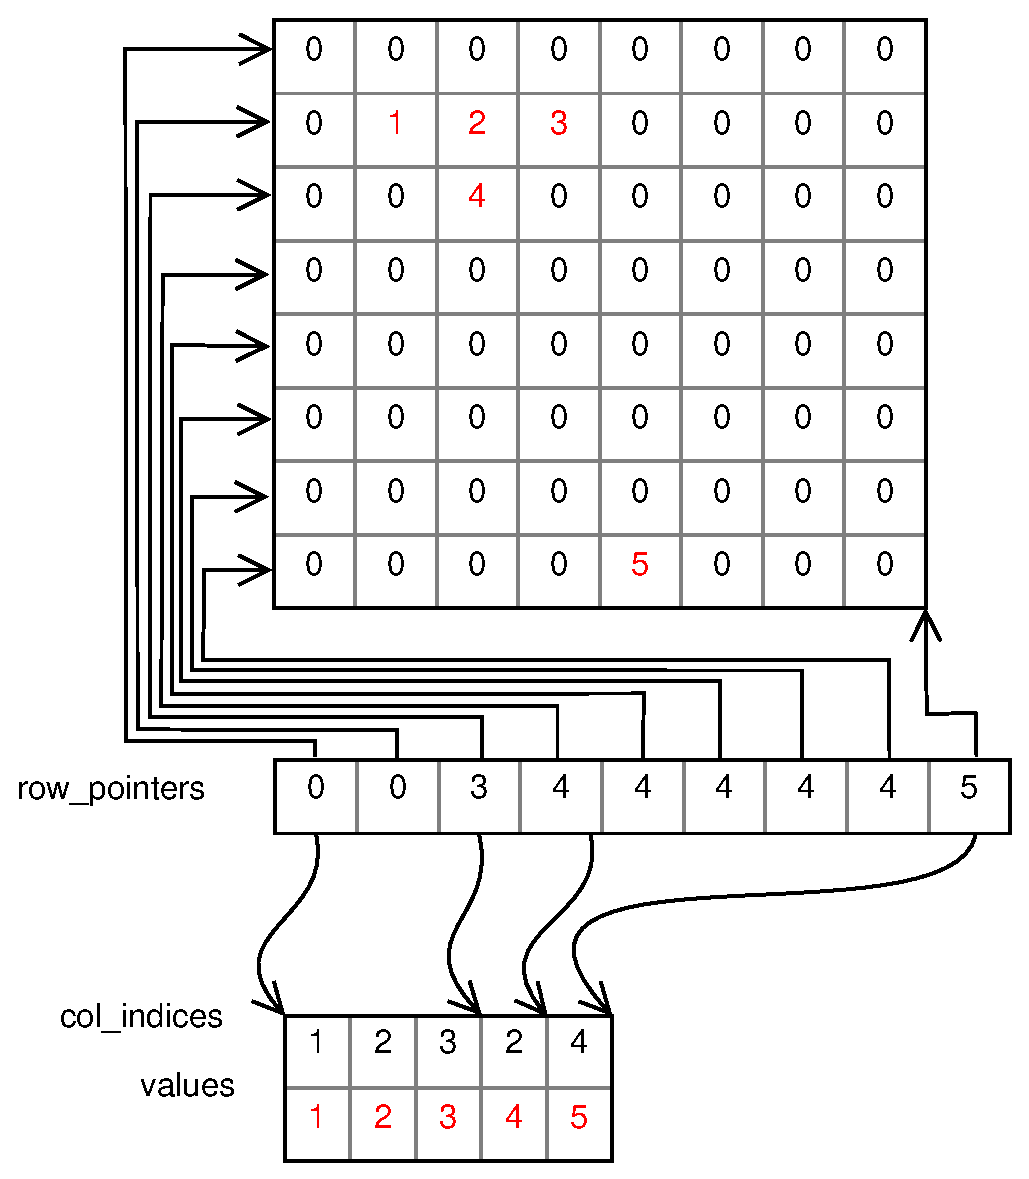
\includegraphics[width=\textwidth]{./images/csr/csr}
	\caption{Matice uložená ve formátu CSR}
	\label{fig:CSR}
\end{figure}


\begin{algorithm}[H]
	\caption{Násobení matice CSR s vektorem}\label{csr-mvm}
	\begin{algorithmic}[1]
		\Procedure{CSR-MVM}{$CSR,V,C$}
		\For{\texttt{$i\gets0$\TO$CSR.h$}}
			\For{\texttt{$ci\gets CSR.rp[i]$\TO$CSR.rp[i + 1]$}}
				\State \texttt{$C.v[r] \gets C.v[r] + CSR.v[ci] * V.v[A.ci[ci]];$}
			\EndFor
		\EndFor
		\EndProcedure
	\end{algorithmic}
\end{algorithm}

\begin{algorithm}[H]
	\caption{Násobení dvou COO matic}\label{csr-mmm}
	\begin{algorithmic}[1]
		\Procedure{CSR-MMM}{$A,B,C$}
		\For{\texttt{$i\gets0$\TO$A.height$}}\Comment{násobení}
			\For{\texttt{$ac\gets A.rp[r]$\TO$A.rp[r+1]$}}
				\For{\texttt{$bc\gets B.rp[A.ci[ac]]$\TO$B.rp[A.ci[ac]+1]$}}
					\State \texttt{$C.v[r][B.ci[bc]] \gets C.v[r][B.ci[bc]] + A.v[ac] * B.v[bc];$}
				\EndFor
			\EndFor
		\EndFor
		\EndProcedure
	\end{algorithmic}
\end{algorithm}


\section{BSR - Block Sparse Row}

\url{https://software.intel.com/sites/products/documentation/doclib/mkl_sa/11/mklman/GUID-9FCEB1C4-670D-4738-81D2-F378013412B0.htm}



\section{Quadtree}

\section{?}

TODO: tady jsem chtel spocictat kdy  se vyplati mit ridkou matici, ale lepsi bude tabulka. Pokud například uložíme matici o rozměrech 100x100 v dvojté přestnosti, bude zabírat \texttt{M x N x sizeof(double) = 100 x 100 x 8 = 80000B = 80kB}. Pokud zvolíme řídký formát matice, kde ke každému elementu uložíme i jeho x a y souřadnici, tak do 80kB uložíme \texttt{80000 / (sizeof(int)+sizeof(int)+sizeof(double)) = 80000/16= 5000} elementů. Pokud matice obsahuje více jak 50  \% nulových elementů, vyplatí se nám ji uložit do řídkého formátu.

%-----------------------------------------------------------------------------

\chapter{Modifikace formátu quadtree}

je to samostatnej bod v zadani tak by to mohla byt cela chapter

TODO: popsat nevyhody quadtree a obrazkama ukazat jak to udelat lip

neco jako quadtree loop unrolling


\chapter{Analýza a návrh}

\section{Práce s řídkými maticemi v moderním software}

\subsection{SciPy.sparse}

SciPy je knihovna skriptovacího jazyka Python.

ZDROJ: \url{http://docs.scipy.org/doc/scipy/reference/sparse.html}


\subsection{Wolfram Mathematica}

Wolfram Mathematica je TODO

Pomocí Wolfram Mathematicy vizualizujeme řídké matice z formátu \texttt{.mtx}. MatrixMarket nabízí matice v souborech \texttt{.mtx.gz} Wolfram Mathematica umí pracovat i s těmito komprimovanými soubory. Příkaz pro importování řídké matice a její vizualizaci je \texttt{Import["/tmp/matrix2.mtx", "Graphics"]}

\url{http://reference.wolfram.com/mathematica/ref/format/MTX.html}


\subsection{Boost}

\url{http://www.boost.org/doc/libs/1_55_0/libs/numeric/ublas/doc/matrix_sparse.htm}


TODO: moznosti implementace, zvolene reseni, ostatni reseni

\chapter{Realizace}

\subsection{Pseudokódy}

(XXX: ?) Pro pseudokódy v této práci platí, že pole jsou indexovaná od nuly a for cyklus $for i \gets 0 to 10$ bude iterovat do devátého prvku. 

\section{MatrixMarket}

TODO: posat format matrixmarket

\subsection{Generátor řídkých matic}

\begin{algorithm}[H]
	\caption{Generování řídkých matic}\label{mmm-recursive}
	\begin{algorithmic}[1]
		\Procedure{SparseMatrixGenerator}{$file,width,height,ItemList$}
		\State \texttt{$MtxWrapper \gets InitMtxWrapper();$}
		\State \texttt{$MtxWrapper.PositionVector \gets InitVector();$}	
		\ForAll{\texttt{$Item \in ItemList$}}
			\State \texttt{$MtxWrapper.addItem(Item.y, Item.x, Item.properties);$}
			\If{$Item.type == Mirrored$}
				\State \texttt{$MtxWrapper.addItem(Item.x, Item.y, Item.properties);$}
			\EndIf
		\EndFor
		\State \texttt{$MtxWrapper.PositionVector.sort();$}
		\State \texttt{$MtxWrapper.PositionVector.removeDuplicates();$}
		\State \texttt{$MtxWrapper.write(file);$}
		\EndProcedure
	\end{algorithmic}
\end{algorithm}

Generátor řídkých matic byl implementován v jednom souboru. Lze spouštět s následujícími parametry:

\begin{itemize}
	\item \texttt{-c} matice bude obsahovat hlavní diagonálu
	\item \texttt{-H <celé číslo>} výška matice
	\item \texttt{-i <typ,a,b,c,d,...>} seznam objektů, které se do matice přidají
	\begin{itemize}
	\item \texttt{diagonal,ay,ax,by,bx,sparsity} prvky v přímce od bodu \texttt{[ax,ay]} do bodu \texttt{[bx,by]} s řídkostí \texttt{sparsity}
	\item \texttt{block,ay,ax,by,bx,sparsity} blok prvků v obdelníku ohraničiného body \texttt{[ax,ay]} a \texttt{[bx,by]} s řídkostí \texttt{sparsity}
	\end{itemize}
	\item \texttt{-n <celé číslo>} velikost matice
	\item \texttt{-o <soubor>} cílový soubor (lze použít i stdout)
	\item \texttt{-s <desetinné číslo>} řídkost matice (\texttt{sparsity})
	\item \texttt{-S <desetine číslo>} startovací číslo
	\item \texttt{-W <celé číslo>} šířka matice
\end{itemize}

\begin{itemize}
	\item \texttt{-h} zobraz nápovědu
	\item \texttt{-o <soubor>} cílový soubor (lze použít i \texttt{stdout}) 
	\item \texttt{-v} vypisuj průběh generování (\texttt{verbose})
\end{itemize}

\texttt{$ ./tests/bin/matrix_generator -n 8192 -s 0.00001 -i mdiagonal,150,0,8192,8042,0.95,mdiagonal,200,10,4000,3000,0.75,mblockwh,300,1500,256,256,0.95,mblockwh,700,2000,128,128,0.95,mrblocks,10,128,64,64,0.75 -o /tmp/matrix2.mtx$}

\begin{figure}[H]
	\includegraphics[width=1.0\textwidth]{./images/generated_matrix}
	\caption{Matice vygenerovaná generátorem}
	\label{fig:aftOrsirr1}
\end{figure}



\section{Optimalizace}

TODO: popsat moznosti optimalizace

\section{? Design implementace}

TODO: C, testy

\section{Měření}

TODO: popsat jak to budu měřit, tedy cas z omp a cachegrind/callgrind


%%%%%%%%%%%%%%%%%%%%%%%%%%%%%%%%%%%%%%%%%%%%%%%%%%%%%%%%%%%%%%%%%%%%%%%%%%%%%%
%%%%%%%%%%%%%%%%%%%%%%%%%%%%%%%%%%%%%%%%%%%%%%%%%%%%%%%%%%%%%%%%%%%%%%%%%%%%%%
%%%%%%%%%%%%%%%%%%%%%%%%%%%%%%%%%%%%%%%%%%%%%%%%%%%%%%%%%%%%%%%%%%%%%%%%%%%%%%
%%%%%%%%%%%%%%%%%%%%%%%%%%%%%%%%%%%%%%%%%%%%%%%%%%%%%%%%%%%%%%%%%%%%%%%%%%%%%%
%%%%%%%%%%%%%%%%%%%%%%%%%%%%%%%%%%%%%%%%%%%%%%%%%%%%%%%%%%%%%%%%%%%%%%%%%%%%%%
%%%%%%%%%%%%%%%%%%%%%%%%%%%%%%%%%%%%%%%%%%%%%%%%%%%%%%%%%%%%%%%%%%%%%%%%%% end
%%%%%%%%%%%%%%%%%%%%%%%%%%%%%%%%%%%%%%%%%%%%%%%%%%%%%%%%%%%%%%%%%%%%%%%%%%%%%%
%%%%%%%%%%%%%%%%%%%%%%%%%%%%%%%%%%%%%%%%%%%%%%%%%%%%%%%%%%%%%%%%%%%%%%%%%%%%%%
%%%%%%%%%%%%%%%%%%%%%%%%%%%%%%%%%%%%%%%%%%%%%%%%%%%%%%%%%%%%%%%%%%%%%%%%%%%%%%
%%%%%%%%%%%%%%%%%%%%%%%%%%%%%%%%%%%%%%%%%%%%%%%%%%%%%%%%%%%%%%%%%%%%%%%%%%%%%%
%%%%%%%%%%%%%%%%%%%%%%%%%%%%%%%%%%%%%%%%%%%%%%%%%%%%%%%%%%%%%%%%%%%%%%%%%%%%%%

%\chapter{Cíl práce}

%\chapter{Analýza a návrh}

%\chapter{Realizace}

\begin{conclusion}
	%sem napište závěr Vaší práce
\end{conclusion}

\bibliographystyle{csn690}
\bibliography{mybibliographyfile}

\appendix

\chapter{Seznam použitých zkratek}
% \printglossaries
\begin{description}
	\item[GUI] Graphical user interface
	\item[XML] Extensible markup language
\end{description}

\nopagebreak[4]
\nopagebreak[4]

% !nesro
\listoffigures

\nopagebreak[4]
\nopagebreak[4]

\listofalgorithms*
% !!nesro

\nopagebreak[4]
\nopagebreak[4]

% % % % % % % % % % % % % % % % % % % % % % % % % % % % 
% % Tuto kapitolu z výsledné práce ODSTRAŇTE.
% % % % % % % % % % % % % % % % % % % % % % % % % % % % 
% 
% \chapter{Návod k~použití této šablony}
% 
% Tento dokument slouží jako základ pro napsání závěrečné práce na Fakultě informačních technologií ČVUT v~Praze.
% 
% \section{Výběr základu}
% 
% Vyberte si šablonu podle druhu práce (bakalářská, diplomová), jazyka (čeština, angličtina) a kódování (ASCII, \mbox{UTF-8}, \mbox{ISO-8859-2} neboli latin2 a nebo \mbox{Windows-1250}). 
% 
% V~české variantě naleznete šablony v~souborech pojmenovaných ve formátu práce\_kódování.tex. Typ může být:
% \begin{description}
% 	\item[BP] bakalářská práce,
% 	\item[DP] diplomová (magisterská) práce.
% \end{description}
% Kódování, ve kterém chcete psát, může být:
% \begin{description}
% 	\item[UTF-8] kódování Unicode,
% 	\item[ISO-8859-2] latin2,
% 	\item[Windows-1250] znaková sada 1250 Windows.
% \end{description}
% V~případě nejistoty ohledně kódování doporučujeme následující postup:
% \begin{enumerate}
% 	\item Otevřete šablony pro kódování UTF-8 v~editoru prostého textu, který chcete pro psaní práce použít -- pokud můžete texty s~diakritikou normálně přečíst, použijte tuto šablonu.
% 	\item V~opačném případě postupujte dále podle toho, jaký operační systém používáte:
% 	\begin{itemize}
% 		\item v~případě Windows použijte šablonu pro kódování \mbox{Windows-1250},
% 		\item jinak zkuste použít šablonu pro kódování \mbox{ISO-8859-2}.
% 	\end{itemize}
% \end{enumerate}
% 
% 
% V~anglické variantě jsou šablony pojmenované podle typu práce, možnosti jsou:
% \begin{description}
% 	\item[bachelors] bakalářská práce,
% 	\item[masters] diplomová (magisterská) práce.
% \end{description}
% 
% \section{Použití šablony}
% 
% Šablona je určena pro zpracování systémem \LaTeXe{}. Text je možné psát v~textovém editoru jako prostý text, lze však také využít specializovaný editor pro \LaTeX{}, např. Kile.
% 
% Pro získání tisknutelného výstupu z~takto vytvořeného souboru použijte příkaz \verb|pdflatex|, kterému předáte cestu k~souboru jako parametr. Vhodný editor pro \LaTeX{} toto udělá za Vás. \verb|pdfcslatex| ani \verb|cslatex| \emph{nebudou} s~těmito šablonami fungovat.
% 
% Více informací o~použití systému \LaTeX{} najdete např. v~\cite{wikilatex}.
% 
% \subsection{Typografie}
% 
% Při psaní dodržujte typografické konvence zvoleného jazyka. České \uv{uvozovky} zapisujte použitím příkazu \verb|\uv|, kterému v~parametru předáte text, jenž má být v~uvozovkách. Anglické otevírací uvozovky se v~\LaTeX{}u zadávají jako dva zpětné apostrofy, uzavírací uvozovky jako dva apostrofy. Často chybně uváděný symbol "{} (palce) nemá s~uvozovkami nic společného.
% 
% Dále je třeba zabránit zalomení řádky mezi některými slovy, v~češtině např. za jednopísmennými předložkami a spojkami (vyjma \uv{a}). To docílíte vložením pružné nezalomitelné mezery -- znakem \texttt{\textasciitilde}. V~tomto případě to není třeba dělat ručně, lze použít program \verb|vlna|.
% 
% Více o~typografii viz \cite{kobltypo}.
% 
% \subsection{Obrázky}
% 
% Pro umožnění vkládání obrázků je vhodné použít balíček \verb|graphicx|, samotné vložení se provede příkazem \verb|\includegraphics|. Takto je možné vkládat obrázky ve formátu PDF, PNG a JPEG jestliže používáte pdf\LaTeX{} nebo ve formátu EPS jestliže používáte \LaTeX{}. Doporučujeme preferovat vektorové obrázky před rastrovými (vyjma fotografií).
% 
% \subsubsection{Získání vhodného formátu}
% 
% Pro získání vektorových formátů PDF nebo EPS z~jiných lze použít některý z~vektorových grafických editorů. Pro převod rastrového obrázku na vektorový lze použít rasterizaci, kterou mnohé editory zvládají (např. Inkscape). Pro konverze lze použít též nástroje pro dávkové zpracování běžně dodávané s~\LaTeX{}em, např. \verb|epstopdf|.
% 
% \subsubsection{Plovoucí prostředí}
% 
% Příkazem \verb|\includegraphics| lze obrázky vkládat přímo, doporučujeme však použít plovoucí prostředí, konkrétně \verb|figure|. Například obrázek \ref{fig:float} byl vložen tímto způsobem. Vůbec přitom nevadí, když je obrázek umístěn jinde, než bylo původně zamýšleno -- je tomu tak hlavně kvůli dodržení typografických konvencí. Namísto vynucování konkrétní pozice obrázku doporučujeme používat odkazování z~textu (dvojice příkazů \verb|\label| a \verb|\ref|).
% 
% \begin{figure}\centering
% 	\includegraphics[width=0.5\textwidth, angle=30]{cvut-logo-bw}
% 	\caption[Příklad obrázku]{Ukázkový obrázek v~plovoucím prostředí}\label{fig:float}
% \end{figure}
% 
% \subsubsection{Verze obrázků}
% 
% % Gnuplot BW i barevně
% Může se hodit mít více verzí stejného obrázku, např. pro barevný či černobílý tisk a nebo pro prezentaci. S~pomocí některých nástrojů na generování grafiky je to snadné.
% 
% Máte-li například graf vytvořený v programu Gnuplot, můžete jeho černobílou variantu (viz obr. \ref{fig:gnuplot-bw}) vytvořit parametrem \verb|monochrome dashed| příkazu \verb|set term|. Barevnou variantu (viz obr. \ref{fig:gnuplot-col}) vhodnou na prezentace lze vytvořit parametrem \verb|colour solid|.
% 
% \begin{figure}\centering
% 	\includegraphics{gnuplot-bw}
% 	\caption{Černobílá varianta obrázku generovaného programem Gnuplot}\label{fig:gnuplot-bw}
% \end{figure}
% 
% \begin{figure}\centering
% 	\includegraphics{gnuplot-col}
% 	\caption{Barevná varianta obrázku generovaného programem Gnuplot}\label{fig:gnuplot-col}
% \end{figure}
% 
% 
% \subsection{Tabulky}
% 
% Tabulky lze zadávat různě, např. v~prostředí \verb|tabular|, avšak pro jejich vkládání platí to samé, co pro obrázky -- použijte plovoucí prostředí, v~tomto případě \verb|table|. Například tabulka \ref{tab:matematika} byla vložena tímto způsobem.
% 
% \begin{table}\centering
% 	\caption[Příklad tabulky]{Zadávání matematiky}\label{tab:matematika}
% 	\begin{tabular}{|l|l|c|c|}\hline
% 		Typ		& Prostředí		& \LaTeX{}ovská zkratka	& \TeX{}ovská zkratka	\tabularnewline \hline \hline
% 		Text		& \verb|math|		& \verb|\(...\)|	& \verb|$...$|		\tabularnewline \hline
% 		Displayed	& \verb|displaymath|	& \verb|\[...\]|	& \verb|$$...$$|	\tabularnewline \hline
% 	\end{tabular}
% \end{table}
% 
% % % % % % % % % % % % % % % % % % % % % % % % % % % % 

\chapter{Obsah přiloženého CD}

%upravte podle skutecnosti

\begin{figure}
	\dirtree{%
		.1 readme.txt\DTcomment{stručný popis obsahu CD}.
		.1 exe\DTcomment{adresář se spustitelnou formou implementace}.
		.1 src.
		.2 impl\DTcomment{zdrojové kódy implementace}.
		.2 thesis\DTcomment{zdrojová forma práce ve formátu \LaTeX{}}.
		.1 text\DTcomment{text práce}.
		.2 thesis.pdf\DTcomment{text práce ve formátu PDF}.
		.2 thesis.ps\DTcomment{text práce ve formátu PS}.
	}
\end{figure}

\end{document}
